\section{Six asymptotic sectors}\label{sec:sectors}

Set
\[
 T=\langle a,b,c\mid aba=bab,\ bcb=cbc,\ cac=aca\rangle,\qquad
 \mathcal E=\{(a,b),(b,c),(c,a)\},
\]
and write \(z_{uv}=(uv)^3\) for \((u,v)\in\mathcal E\).

\begin{proposition}\label{prop:triangle-obstruction}
There is no geometric action of \(T\) such that, for every
\((u,v)\in\mathcal E\),
\begin{equation}\label{eq:strict-ratios}
 \frac{\ell(z_{uv})}{3\ell(u^2)}
 =\frac{\ell(z_{uv})}{3\ell(v^2)}>\frac12.
\end{equation}
\end{proposition}

The denominators are positive in every geometric action: sending each
of \(a,b,c\) to \(1\in\mathbb Z\) shows that their squares have infinite
order, so Lemma~\ref{lem:semisimple} applies.  The equality of the two
ratios also follows from conjugacy of adjacent braid generators.
We prove the proposition in Section~\ref{sec:localization}.  In this
section, assume for contradiction that such an action on \(Y\) exists
and fix \(y\in Y\).

We will construct a parameter disk \(P\) made of six Euclidean sectors
and maps \(f_n:P\to Y\), indexed by positive integers \(n\).  Within
each sector, image distances divided by \(n\) approach Euclidean
distances.  Mirror coordinates will ensure a second property: disjoint
closed regions of \(P\) have images separated by a positive multiple
of \(n\).  The total sector angle below \(2\pi\) then lets us fill the
same boundary by a second disk whose image stays a positive multiple
of \(n\) from \(y\).  Sections~\ref{sec:diagrams} and
\ref{sec:localization} compare the resulting sphere with finite labelled
diagrams to obtain the contradiction.

\subsection{Orbit control and mirror coordinates}

Let \(d_T\) be the word metric for \(a,b,c\) and their inverses.
The following form of the \v{S}varc--Milnor orbit comparison is standard;
see \cite[I.8.18--19]{BridsonHaefliger1999}.  Its direct proof records
the constants used to turn mirror-coordinate separation into metric
separation.

\begin{lemma}\label{lem:orbit-control}
For a geometric action of \(T\) and any base point \(y\), there are
constants \(R,C<\infty\) such that \(Ty\) is \(R\)-dense and
\begin{equation}\label{eq:orbit-control}
 d_T(s,t)\le C\bigl(1+d_Y(sy,ty)\bigr)\qquad(s,t\in T).
\end{equation}
\end{lemma}

\begin{proof}
If \(TK=Y\) with \(K\) compact, take
\(R=\max_{p\in K}d(y,p)\).  Every \(tp\) is within \(R\) of \(ty\).
For \(L=d(sy,ty)\), divide the geodesic into
\(N=\max(1,\lceil L\rceil)\le L+1\) pieces, each of length at most one.
Choose nearby orbit points at the division points, keeping the prescribed
endpoint labels \(s,t\).  Each successive group increment \(q\) satisfies
\(d(y,qy)\le2R+1\).  There are finitely many such \(q\): the compact ball
\(\overline B(y,2R+1)\) contains both \(y\) and \(qy\), so properness
applies.  The largest word length of these increments, enlarged to at
least one, can be used for \(C\).  Summing their word lengths proves
\eqref{eq:orbit-control}.
\end{proof}

Digne's reflection-coordinate homomorphism sends an Artin generator
associated to a reflection \(r\) to \((e_r,r)\) in a semidirect product
\cite[Proposition~2.1]{Digne2016}.  We use its concrete version for the
side reflections of an equilateral triangle and verify its formulas.
The resulting coordinates will distinguish all six sectors.

Take an equilateral triangle in the Euclidean plane, and denote its
three side lines by \(D_a,D_b,D_c\).  Let \(r_u\) be reflection in
\(D_u\), and let \(\mathcal D\) be the set of all images of these three
lines under the generated reflection group.  Write
\[
 E=\bigoplus_{D\in\mathcal D}\mathbb R e_D,\qquad
 \left\|\sum_D \xi_D e_D\right\|_1=\sum_D|\xi_D|.
\]
All vectors here have finite support.  Each \(r_u\) preserves
\(\mathcal D\) and acts linearly on \(E\) by permuting its basis vectors.

\begin{lemma}\label{lem:mirror-action}
The formulas
\[
 u\cdot\xi=e_{D_u}+r_u\xi\qquad(u=a,b,c)
\]
define an affine isometric action of \(T\) on \(E\).  If \(V(t)=t\cdot0\),
then
\begin{equation}\label{eq:mirror-lipschitz}
 \|V(t)-V(s)\|_1\le d_T(s,t).
\end{equation}
For each \((u,v)\in\mathcal E\), the elements \(u^2,z_{uv}\) act by pure
translations with vectors
\begin{equation}\label{eq:mirror-translations}
 L_u=2e_{D_u},\qquad
 L_{uv}=2(e_{D_u}+e_{D_v}+e_{D_{uv}}),
\end{equation}
where \(D_{uv}\) is the third mirror at \(D_u\cap D_v\).
The three lines \(D_{ab},D_{bc},D_{ca}\) are distinct from one another
and from \(D_a,D_b,D_c\).
\end{lemma}

\begin{proof}
Two incident side reflections generate the reflection group of three
lines spaced at angles \(\pi/3\) about their intersection.  Their two
length-three braid words have the same linear part.  The translation
part of \(uvu\) is
\[
 e_{D_u}+e_{r_uD_v}+e_{r_ur_vD_u}
 =e_{D_u}+e_{D_{uv}}+e_{D_v}.
\]
For \(vuv\), the three terms occur in the reverse order.  Thus the
translation parts also agree, proving the affine braid relations.

Each generator or inverse moves \(0\) a vector of norm one, so a word
of length \(k\) moves \(0\) a distance at most \(k\).  For the linear
permutation part \(r_s\) of \(s\), the cocycle identity gives
\[
 V(t)-V(s)=r_s V(s^{-1}t).
\]
Taking norms proves \eqref{eq:mirror-lipschitz}.

Reflection in \(D_u\) fixes its own basis vector, giving the translation
vector \(2e_{D_u}\) for \(u^2\).  Also
\((uv)^3=(uvu)^2\).  The affine map \(uvu\) has translation vector equal
to the sum of the three mirror vectors, and its linear part preserves
that sum and has square one.  Squaring proves the second formula in
\eqref{eq:mirror-translations}.  The third mirror at a vertex of an
equilateral triangle is parallel to the opposite side and distinct from
it.  The three opposite directions are different.  This proves the
last assertion.
\end{proof}

\subsection{The parameter disk}

For each pair \((u,v)\in\mathcal E\), use both commuting pairs
\[
 (U,H)=(u^2,z_{uv}),\qquad (U,H)=(v^2,z_{uv}).
\]
Commutation follows from Lemma~\ref{lem:braid-centers}.
On the exponent plane \(\mathbb R^2\) of each pair, let
\(\|\cdot\|_{U,H}\) be the stable seminorm from
Lemma~\ref{lem:commuting-form}.  Give its nonnegative quadrant exponent
coordinates \((\lambda,\mu)\), corresponding to \(U,H\), respectively.
The next lemma proves that this quadrant is a Euclidean sector.

\begin{lemma}\label{lem:sector-data}
Each of these six seminorms is positive definite.  Each sector angle
\(\theta\) satisfies \(0<\theta<\pi/3\).
The sectors glue isometrically along their shared rays, in the cyclic
order
\begin{equation}\label{eq:ray-order}
 a^2,\ z_{ab},\ b^2,\ z_{bc},\ c^2,\ z_{ca},\ a^2.
\end{equation}
Their radius-one disk \(P\) is a topological disk with total angle
\(0<\Omega<2\pi\).  It has a continuous injective map \(v_*:P\to E\)
whose value in a sector for \(U=u^2,H=z_{uv}\) is
\begin{equation}\label{eq:separating-coordinates}
 v_*(\lambda,\mu)=\lambda L_u+\mu L_{uv},
\end{equation}
and similarly with \(v\) in place of \(u\).
\end{lemma}

\begin{proof}
For integral \((i,j)\), the pure translation formulas give
\[
 V((U^iH^j)^m)=m(iL_u+jL_{uv}).
\]
Use \eqref{eq:mirror-lipschitz} and \eqref{eq:orbit-control}, divide by
\(m\), and let \(m\to\infty\).  It follows that
\[
 \|iL_u+jL_{uv}\|_1\le C\|(i,j)\|_{U,H}.
\]
The same inequality holds on rational vectors by homogeneity and on
real vectors by continuity.  The two displayed translation vectors are
linearly independent: the extra-mirror coordinate first determines
\(j\), and the \(D_u\)-coordinate then determines \(i\).
The stable form is therefore positive definite.

The central pairing formula
\eqref{eq:braid-central-pairing}, with \(r=3\), gives
\[
 \langle U,H\rangle=\frac{\ell(H)^2}{3}.
\]
Hence
\begin{equation}\label{eq:sector-angle}
 \cos\theta=\frac{\langle U,H\rangle}{\ell(U)\ell(H)}
 =\frac{\ell(H)}{3\ell(U)}>\frac12.
\end{equation}
Positive definiteness ensures \(\cos\theta<1\).
This proves the angle bounds.

Along a ray for an element \(W\), exponent \(t\ge0\) has distance
\(t\ell(W)\) from the origin in either adjacent sector.  Thus the
identifications preserve both exponents and metrics.
The resulting cone is parametrized by a radius \(r\ge0\) and a cyclic
angle of period \(\Omega\), with all angle values identified at \(r=0\).
Its part \(0\le r\le1\) is the asserted disk.

The formulas for \(v_*\) agree on every shared ray.  If a vector in its
image has a nonzero extra-mirror coordinate, that coordinate specifies
\((u,v)\) and \(\mu\).  The excess over \(2\mu\) on one of the original
two side coordinates specifies the remaining exponent and which of
the two sectors is used.  If there is no excess, the point is on the
shared \(H\)-ray.  With no extra-mirror coefficient, the vector is on
one squared-generator ray or is zero.  These descriptions distinguish
points precisely up to the stated ray identifications.  They prove
injectivity, including at the origin.
\end{proof}

We use only the Euclidean metric within each sector of \(P\);
we do not claim that this cone disk is CAT(0).
Figure~\ref{fig:sectors} shows the cyclic gluing.

\begin{figure}[htbp]
 \centering
 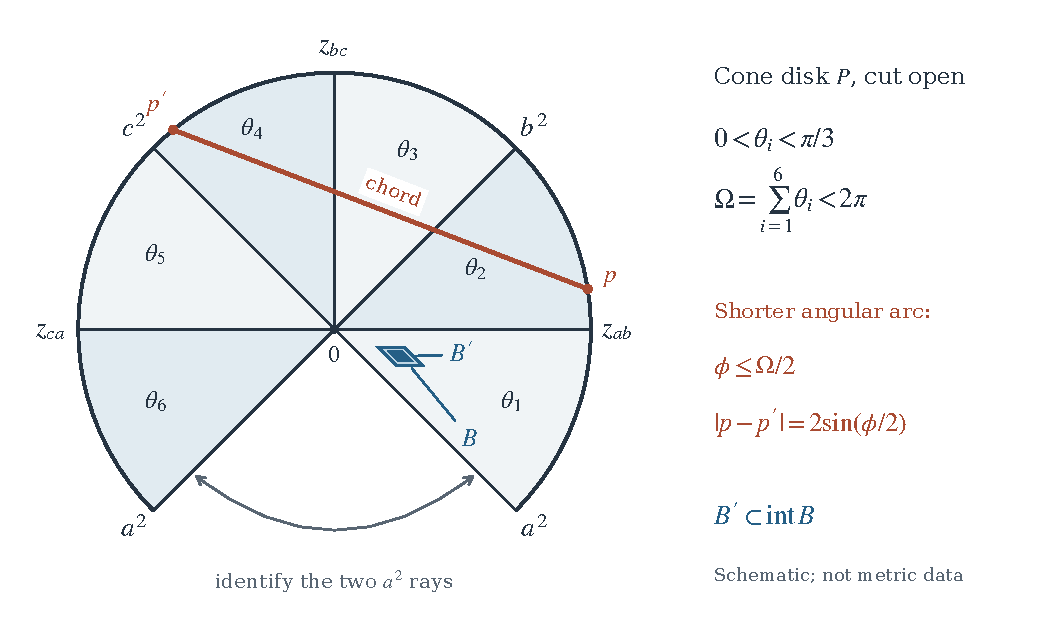
\includegraphics[width=.82\textwidth]{figures/sectors.pdf}
 \caption{The six sectors of the parameter disk \(P\), cut open along
 the \(a^2\)-ray.
 The two boundary copies of that ray are identified.  The angles and patch sizes are
 schematic; each angle is less than \(\pi/3\), with total \(\Omega<2\pi\).
 The chord is drawn after unfolding a shorter angular arc and illustrates
 Lemma~\ref{lem:outer-cap}; the nested patches
 \(B'\subset\operatorname{int}B\) are chosen in
 Subsection~\ref{sec:local-patch} for the local winding count.}
 \label{fig:sectors}
\end{figure}

\subsection{Uniform asymptotic maps}

In each sector define the group label
\begin{equation}\label{eq:sector-label}
 t_n(p)=U^{\lfloor n\lambda\rfloor}H^{\lfloor n\mu\rfloor}.
\end{equation}
These labels agree on the glued rays.

\begin{samepage}
\begin{lemma}\label{lem:sector-maps}
There are continuous maps \(f_n:P\to Y\), with \(f_n(0)=y\), and a
constant \(C_0\) independent of \(n,p\), such that
\begin{equation}\label{eq:grid-error}
 d_Y(f_n(p),t_n(p)y)\le C_0.
\end{equation}
For two points in any one sector,
\begin{equation}\label{eq:sector-convergence}
 \frac{d_Y(f_n(p),f_n(p'))}{n}
 \longrightarrow\|p-p'\|_{U,H}
\end{equation}
uniformly.  In addition, uniformly on \(P\),
\begin{equation}\label{eq:radial-coordinates}
 \frac{d_Y(y,f_n(p))}{n}\longrightarrow r(p),
 \qquad
 \frac{V(t_n(p))}{n}\longrightarrow v_*(p).
\end{equation}
If \(A_1,A_2\subset P\) are disjoint nonempty closed sets, then for
some \(\delta>0\) and all sufficiently large \(n\),
\begin{equation}\label{eq:region-separation}
 d_Y(f_n(A_1),f_n(A_2))\ge\delta n.
\end{equation}
\end{lemma}
\end{samepage}

\begin{proof}
Triangulate the entire exponent quadrant by squares of side \(1/n\),
each split along a diagonal, and assign the vertex \((i/n,j/n)\) the
point \(U^iH^j y\).  Use constant-speed geodesics on edges.  On each
triangle, cone the opposite edge to its remaining vertex using geodesics.
This gives a continuous map: all restrictions to common edges are the
same geodesic parametrization.  Geodesic convexity bounds the distance
of every image point from a vertex by the maximum of the corresponding
vertex distances.  Commutation bounds those distances uniformly by
the displacements of \(U,H\).  Restricting to the radius-one sector
therefore gives \eqref{eq:grid-error}.  The restrictions on shared rays
agree, so the six maps glue.  There are only six sectors, allowing a
common \(C_0\).

For one commuting pair put
\[
 F(i,j)=d_Y(y,U^iH^j y)\qquad((i,j)\in\mathbb Z^2).
\]
The triangle inequality and commutation give
\[
 |F(i,j)-F(i',j')|
 \le d(y,Uy)|i-i'|+d(y,Hy)|j-j'|.
\]
For a fixed rational vector \(q=(a/m,b/m)\), compare
\(\lfloor nq\rfloor\) with
\(\lfloor n/m\rfloor(a,b)\); their difference stays bounded.
The definition of stable length consequently gives
\[
 \frac{F(\lfloor nq\rfloor)}n
 \longrightarrow\frac{\ell(U^aH^b)}m=\|q\|_{U,H}.
\]
This includes negative \(a,b\).  On a bounded real region, choose a
finite rational net of arbitrarily small mesh.  The common Lipschitz
bound above, with a rounding error \(O(1/n)\), and continuity of the
stable norm upgrade this convergence to uniform convergence on the
region.

For \(p,p'\) in a sector, the difference between their floored exponent
vectors differs from the floor of \(n(p'-p)\) by a bounded integer
vector.  The orbit distance between their labels is \(F\) of that
difference.  The uniform result and \eqref{eq:grid-error} prove
\eqref{eq:sector-convergence}.  Taking one point to be \(0\) gives the
radial assertion.  The other assertion of \eqref{eq:radial-coordinates}
follows directly from \eqref{eq:mirror-translations}; its error is
in fact \(O(1/n)\).

Finally, compactness and injectivity give
\[
 \eta=\min_{p\in A_1,\ q\in A_2}\|v_*(p)-v_*(q)\|_1>0.
\]
By \eqref{eq:radial-coordinates}, the norm of
\(V(t_n(p))-V(t_n(q))\) is at least \(\eta n/2\), uniformly for these
pairs and large \(n\).  Combining \eqref{eq:mirror-lipschitz},
\eqref{eq:orbit-control}, and \eqref{eq:grid-error} gives
\[
 d_Y(f_n(p),f_n(q))
 \ge\frac{\eta n}{2C}-1-2C_0.
\]
Decreasing the positive coefficient proves
\eqref{eq:region-separation}.
\end{proof}

\begin{lemma}\label{lem:outer-cap}
There is \(\epsilon>0\) such that, for all sufficiently large \(n\),
the map \(f_n|_{\partial P}\) extends to a second parameter disk whose
entire image lies outside \(B_Y(y,\epsilon n)\).
Gluing the two parameter disks gives a continuous sphere map, still
denoted \(f_n\).
\end{lemma}

\begin{proof}
For any two points of \(\partial P\), choose a shorter angular arc
between them.  Its angle \(\phi\) is at most \(\Omega/2<\pi\).
Unfold its sectors to a Euclidean wedge.  The wedge intersected with
the unit disk is convex, so the chord between the points stays within
it, as in Figure~\ref{fig:sectors}.  Its length is
\[
 2\sin(\phi/2)\le2\sin(\Omega/4).
\]
Each sector appears at most once in this development, except that a sector
containing both endpoints may appear in two end pieces.  Each such
piece is convex, so its intersection with the chord is a segment.
The chord therefore splits into at most seven single-sector pieces.  Apply the
uniform estimate \eqref{eq:sector-convergence} to each piece.  Uniformly
for \(p,p'\in\partial P\), this gives
\begin{equation}\label{eq:boundary-short}
 d_Y(f_n(p),f_n(p'))
 \le2\sin(\Omega/4)n+o(n).
\end{equation}

Fix \(p_0\in\partial P\) and cone the boundary map to \(f_n(p_0)\) by
geodesics.  Their continuous dependence makes this a continuous map
of a parameter disk.  If \(q\in[A,B]\), the two triangle inequalities
give
\[
 d(y,q)\ge
 \max\{d(y,A)-d(A,q),\,d(y,B)-d(q,B)\}
 \ge\frac{d(y,A)+d(y,B)-d(A,B)}2.
\]
Here both endpoints have distance \(n+o(n)\) from \(y\), uniformly,
by \eqref{eq:radial-coordinates}; \eqref{eq:boundary-short} bounds their
distance.  The entire coning segment therefore stays at distance at
least
\[
 \bigl(1-\sin(\Omega/4)\bigr)n-o(n)
\]
from \(y\).  Take
\(\epsilon=\tfrac12(1-\sin(\Omega/4))>0\).
\end{proof}
